\documentclass[useAMS,usenatbib]{mn2e}
\usepackage{graphicx}
\usepackage{url}

%\usepackage{tikz}
\newcommand{\aap}{Astron. Astrophys.}
\newcommand{\aj}{Astron. J.}
\newcommand{\ao}{Appl. Opt.}
\newcommand{\apj}{Astrophys. J.}
\newcommand{\apjl}{Astrophys. J. Lett.}
\newcommand{\apjs}{Astrophys. J. Suppl.}
\newcommand{\mnras}{Mon. Not. Roy. Ast. Soc.}
\newcommand{\mn}{Mon. Not. Roy. Ast. Soc.}
\newcommand{\nat}{Nature}
\newcommand{\pasa}{Publ. Ast. Soc. Aust.}
\newcommand{\pasp}{Publ. Ast. Soc. Pac.}
\newcommand{\prl}{Phys. Rev. Lett.}
\newcommand{\prd}{Phys. Rev. D}
\newcommand{\msun}{\mathrm{M}_\odot}

\title[Inpainting]{Inpainting of Galaxy Redshift Surveys}
\author[Caiazzo, Antolini \& Heyl]{Ilaria Caiazzo$^{1}$, Elisa Antolini$^{2}$,  Jeremy S. Heyl$\thanks{Email:
    heyl@phas.ubc.ca; Canada Research Chair}^{1}$ \\
  $^{1}$Department of Physics and Astronomy, University of British
  Columbia, 6224 Agricultural Road, Vancouver, BC V6T 1Z1, Canada\\
  $^{2}$Dipartimento di Fisica e Geologia, Universit\`a degli Studi di Perugia, I-06123 Perugia, Italia \\
}
\begin{document}
\date{Accepted ---. Received ---; in original form ---}

\pagerange{\pageref{firstpage}--\pageref{lastpage}} \pubyear{2016}

\maketitle

\label{firstpage}

\begin{abstract}
\end{abstract}

\section{The Tecnhique}
\label{sec:tecnhique}
The technique is straightforward to describe and to implement, and we
will outline it below.  Let the map be given by $a(\Omega)$ and the
mask by $m(\Omega)$ where $m(\Omega)=1$ where the underlying galaxies
are visible.
\begin{enumerate}
\item
  Set an initial guess for the underlying map.
\begin{equation}
  y_1(\Omega) = \frac{\left \langle  m(\Omega) a(\Omega)  \right \rangle}{\left \langle m(\Omega) \right \rangle }
    \label{eq:2}
\end{equation}
\item
  Calculate the residual of the current guess
  \begin{equation}
    r_t(\Omega) =  m(\Omega) a(\Omega) - y_t(\Omega)
    \label{eq:3}
  \end{equation}
\item
  Expand the sum of the residuals in the unmasked region and the current guess
  in spherical harmonics.
  \begin{equation}
    A_{lm,t} = \int d\Omega Y^*_{lm} \left [ m(\Omega) r_t(\Omega) + y_t(\Omega) \right ]
    \label{eq:4}
  \end{equation}
\item
  Keep only the components with the largest amplitudes and set the
  amplitudes smaller than the threshold ($\lambda_t$) to zero.
\item
  Calculate the new guess from the largest components
  \begin{equation}
    y_{t+1}(\Omega) = \sum_{|A_{lm,t}| > \lambda_t} A_{lm,t} Y_{lm}(\Omega).
    \label{eq:5}
  \end{equation}
\item
  Decrease the threshold $\lambda_t$ and repeat from step (ii) until the stopping criterion
  is reached.
\end{enumerate}
There is of course some art in choosing the size of the underlying
basis, the thresholds and the stopping criterion.  Here we expand the
galaxy map to $l_\mathrm{max}=m_\mathrm{max}=64$, so there are a total
of 2,145 components.  The threshold is set to keep a given fraction of
the components at each step.  The fraction increases from $10^{-3.5}$
to $10^{-0.5}$ over 200 iterations, so the initial representations use
just a few components and the number of components increases to about
680 at the final iteration, so over two thirds of the spherical
harmonic components are set to zero in the final map.

From the iterative procedure above it is apparent that the value of
the guess within the masked region (where $m(\Omega)=0$) does not
contribute to the residual and does not influence the solution.
However, the spherical harmonics that contribute to the data near the
edge of the mask do influence the guess within the masked region.

fake test gives R=0.70

\section{Tests}
\label{sec:tests}


\subsection{Simulated Maps}
\label{sec:simulated-maps}

To understand the effectiveness of these techniques we simulate galaxy
sky maps with the Galactic plane hidden and cross-correlate the
restructed galaxy maps with the original simulated map.  For make the
simulation as realistic as possible we use the angular power spectrum
of the observed galaxy map from 2MASS to construct the test maps.
These simulated maps by design have the same angular power spectrum as
the real 2MASS data including the zone of avoidance but different
phases, so they don't exhibit a zone of avoidance and they lack the
potential higher order correlations that the data may exhibit.
Fig.~\ref{fig:testmap} depicts a particular example of this technique.
We used the angular power spectrum of the upper panel to create one
hundred independent maps with the same power spectrum; one of these is
depicted in the middle panel of the figure.  We masked the Galactic
plane and used the infilling techinique to fill in the region.  The
lower panel depicts the difference between in the infilled map and the
original.
\begin{figure}
  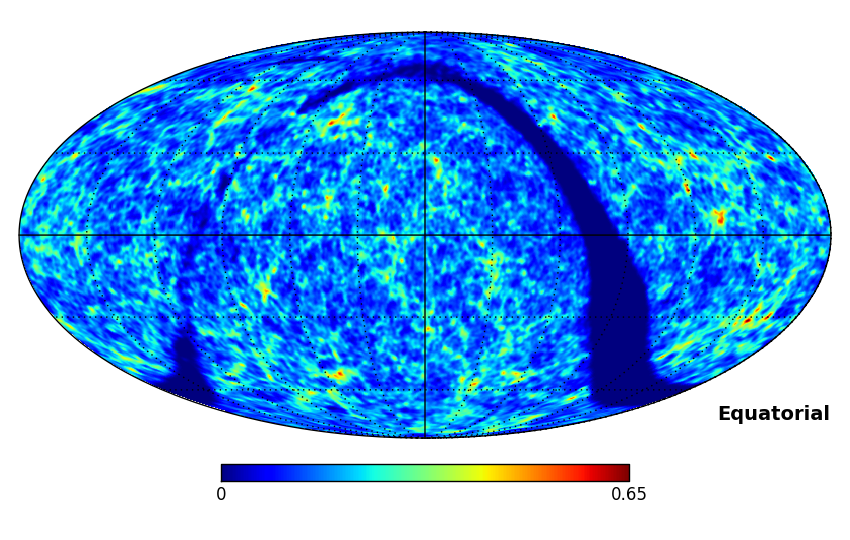
\includegraphics[width=\columnwidth]{cleantest_000/orig_map}
  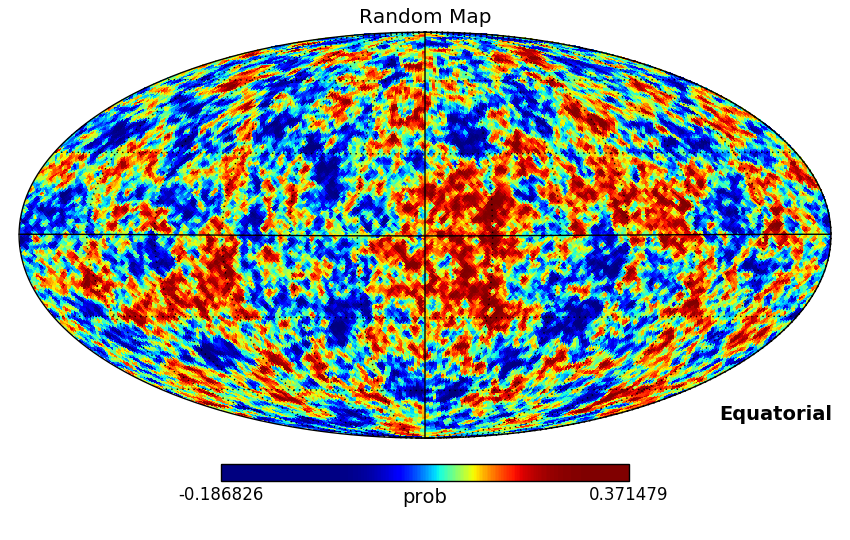
\includegraphics[width=\columnwidth]{cleantest_000/RandMap}
  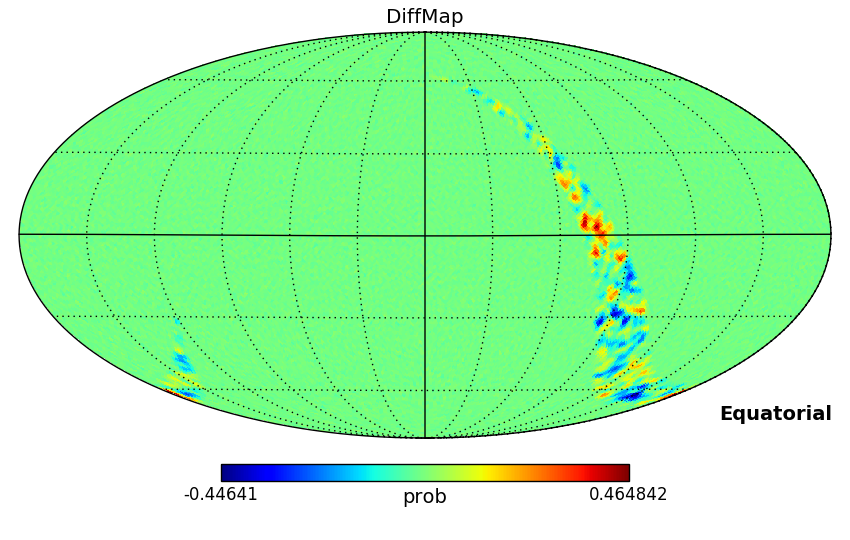
\includegraphics[width=\columnwidth]{cleantest_000/DiffMap}
  \caption{Upper: the relative surface density of galaxies in the
    2-MASS Photometric Redshift Survey with photometric redshifts
    between 0.01 and 0.1, smoothed with a Gaussian of 0.6 degrees
    (0.01 radian), the input map.  Middle: the test map constructed
    using the angular power spectrum of the map in the upper panel.
    Lower: we masked the Galactic plane of the middle panel and
    reconstructed the image using the techinque in
    \S~\ref{sec:tecnhique}.  The difference between the middle panel
    and the reconstructed map is depicted.}
  \label{fig:testmap}
\end{figure}

To make statistic sense of the agreement we calculate Pearson's
correlation coefficient ($r$) between the original data and the
infilled reproductions within the infilled region for each of the
trials and examine its cumulative distribution as depicted in
Fig.~\ref{fig:cleantest}.  The distribution of $r$ is
well-characterized by a normal distribution with mean of $0.267$ and a
standard deviation of $0.10$.  For comparision the correlation
coefficient of the galaxy map with a bootstrapped realisation of the
same map over the test region is typically much higher $r=0.97$, so
clearly much information is lost in the reconstruction, but the test
reveals that the infilling procedure does give a good first-order
guess at the hidden structures.
\begin{figure}
  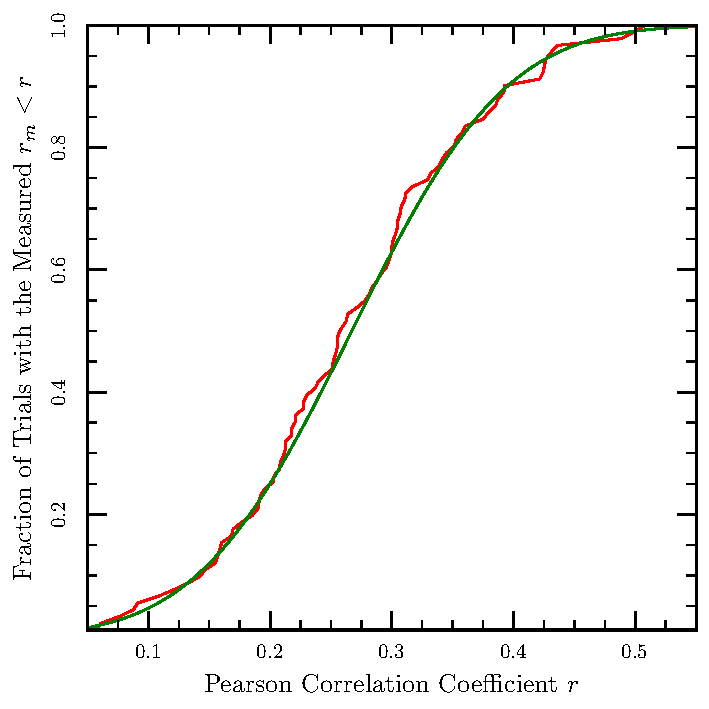
\includegraphics[width=\columnwidth]{cleantest}
  \caption{Cumulative distribution of $r$ for 100 trials of the
    infilling procedure with simulated data in red.  The smooth green
    curve traces the cumulative normal distribution with mean of $0.267$
    and standard derivation of $0.10$.
  }
  \label{fig:cleantest}
\end{figure}

\subsection{Observed Maps}

Here we will discuss in further detail the tests that we performed in
\citet{2016arXiv160207710A}.  To summarize we determine the region
masked by the Galaxy by finding the region in which the density of
galaxies is either less than one tenth of the mean (from the upper
panel of Fig.~\ref{fig:testmap}) or in which the density of stars
\citep[from Fig.~2][]{2016arXiv160207710A} is greater than a threshold
that accounts for the masking of the background galaxies due to the
Large Magellanic Cloud, a feature that is apparent in both figures.
Both of these masks are nearly the same, so we combine them.

To demonstrate its efficacy here, we will first apply the procedure to
a galaxy map that has an additional mask as depicted in
Fig.~\ref{fig:infilling_test}.  We have masked both the Galactic plane
and the equatorial plane.  These equatorial region outside the
Galactic plane is our test region where we know the underlying galaxy
distribution, and we attempt to reconstruct it from the data outside
the masked regions.  Most of the structures within the equatorial
region in the top panel are reproduced in the lower panel.  However,
to make statistic sense of the agreement we calculate Pearson's
correlation coefficient ($r$) between the original data and the
infilled reproduction within the infilled region outside of the
Galactic plane.  We obtain a value of $r=0.25$ about the mean from the
tests in \S~\ref{sec:simulated-maps}.  To estimate the significance of
this value, we performed two tests.  First, we calculated the angular
power spectrum of the original galaxy map and generated 1,000 galaxy
maps consistent with this power spectrum.  The largest obtained was
0.171, and the distribution was consistent with a normal distribution
with $\sigma=0.066$ and zero mean, so the observed correlation over
the test region reaches nearly four-sigma significance.
\begin{figure}
  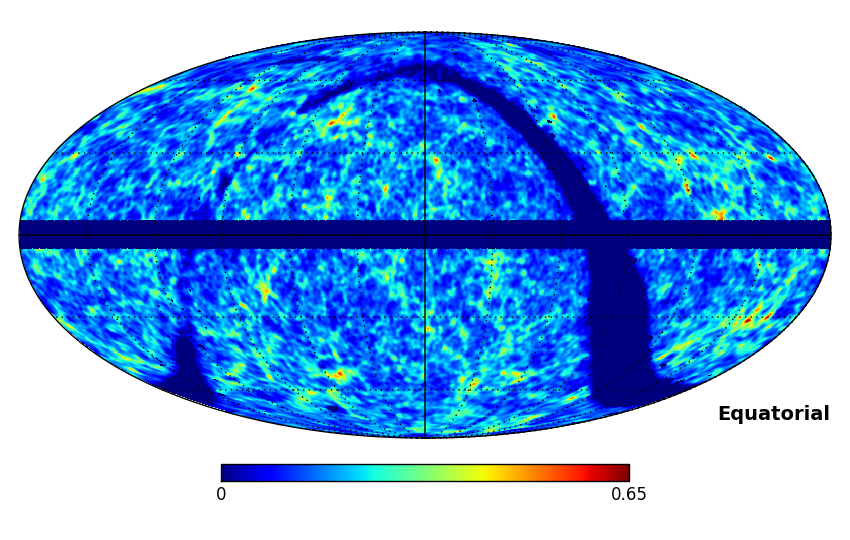
\includegraphics[width=\columnwidth]{infill_test_maskeddataC.png}
  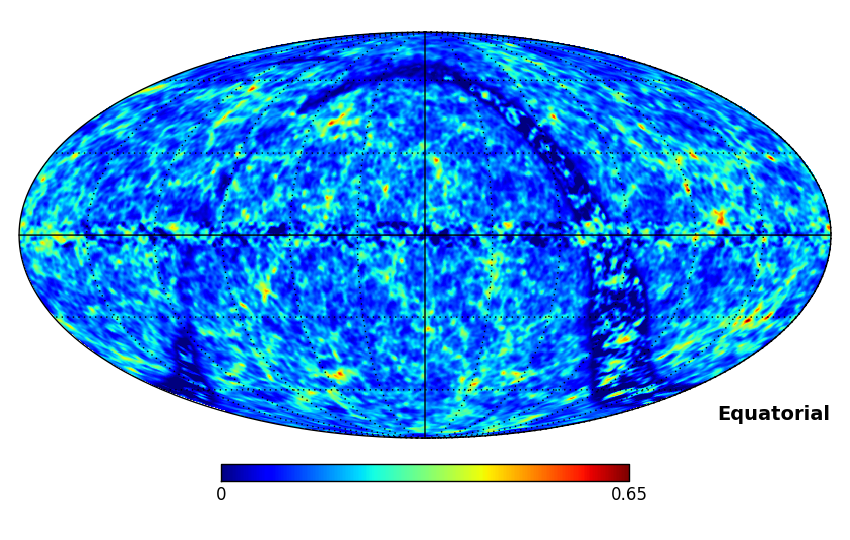
\includegraphics[width=\columnwidth]{infill_test_resultC.png}
  \caption{Upper: we masked both the Galactic plane and within
    five degrees of the celestial equator.  Lower: the infilled galaxy
    distribution both in the Galactic plane and the equatorial plane
    to compare with the upper panel.}
  \label{fig:infilling_test}
\end{figure}

The second test exploited the fact that the mask that we used was a
strip in equatorial coordinates, so if we shift the reconstructed
galaxy map relative to the input map in right ascension, we do not
expect the two maps to be correlated.  This shift test is depicted in
the upper panel of Fig.~\ref{fig:shift_test}.  For zero degrees, the
maximum correlation of $0.25$ is achieved but for shifts greater than
a few degrees the correlation appears to be centered about zero.  The
lower panel gives the cumulative distribution of correlation
coefficients.  The mean is just slightly less than zero and the
standard deviation is $0.04$, slightly less than for the first test.
Again we see than the observed correlation for the unshifted data of
$0.25$ is statistically significant.  The reconstruction contains much
more information about the hidden galaxy distribution that one would
expect by chance.
\begin{figure}
  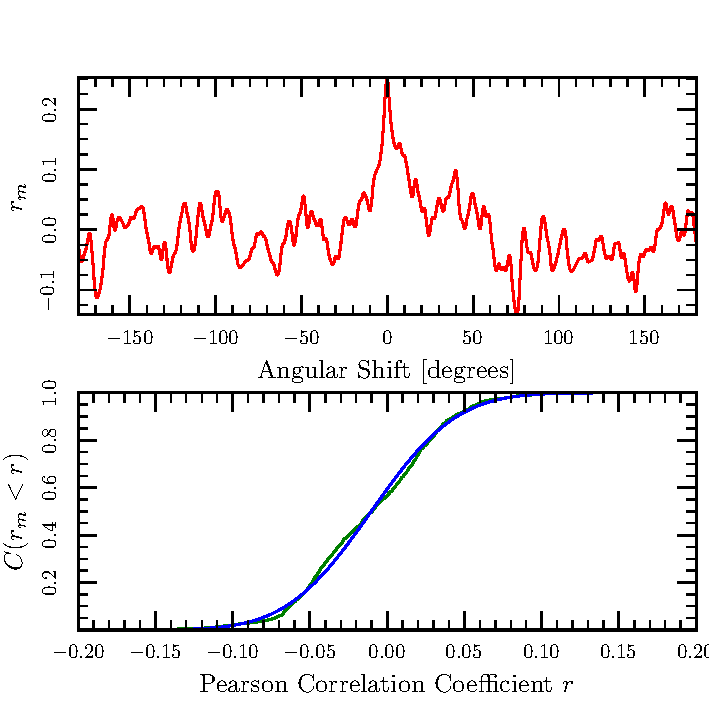
\includegraphics[width=\columnwidth]{ang_combo}
  \caption{Upper panel: The curve depicts the Pearson's correlation
    coefficient as a function of the relative shift between in the
    input map and the reconstuction calculated over the equatorial
    masked region. Lower panel: The green curve tracks the cumulative
    distribution of $r$ for shifts greater than 10 degrees.  The
    smooth blue curve traces the cumulative normal distribution with
    mean of $-0.01$ and standard derivation of $0.04$.}
  \label{fig:shift_test}
\end{figure}

\section{Results}

After demonstrating the efficacy of the infilling procedure, we now
perform the calculation to infill only through the Galactic plane (we
did infill the Galactic plane in the tests as well).  The upper panel
of Fig~\ref{fig:infilling} depicts the mask that we will use to mask
the data.  For the data we will be using the 2MPZ galaxies with redshifts from 0.01 to 0.2 to combine with the zone of avoidance survey of \citet{2016AJ....151...52S} within the same redshift range. The middle
panel gives the initial galaxy map with the masked region filled in.
There are several structures within masked region that connect with
the structures on either side of the Galactic plane.  Finally, we can
estimate the dispersion of the infilled map by calculate a series
of galaxy density maps by resampling the 2MPZ to obtain new
catalogues, new maps and new infilled maps.  The lower panel of
Fig.~\ref{fig:infilling} depicts the dispersion ratio of the map.
Outside of the Galactic plane the signal-to-noise almost everywhere
exceeds four.  In the infilled region most of the overdense structures
correspond to high signal-to-noise regions.
\begin{figure}
  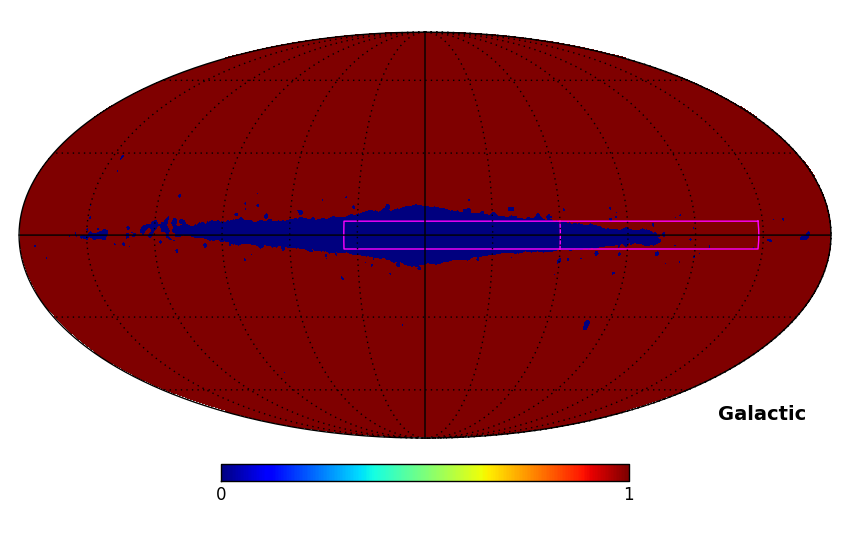
\includegraphics[width=\columnwidth,clip,trim=0 1in 0 0]{prod_mask}
  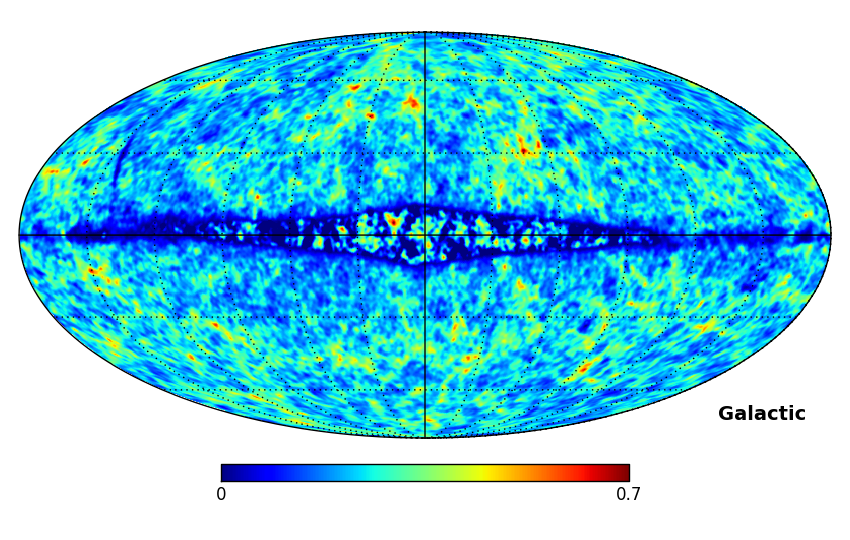
\includegraphics[width=\columnwidth]{infilled_prod_mask}
  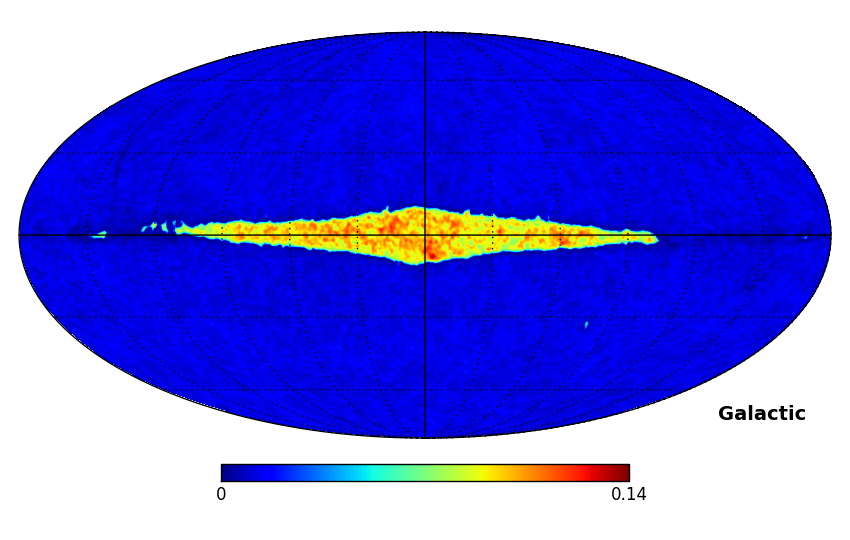
\includegraphics[width=\columnwidth]{sigma_prod_mask}
  \caption{Upper: the mask used for the infilling procedure obtained
    by determining the regions where the galaxy density is less than
    one tenth of the mean or the star density lies above a given
    threshold (see text for details).  Middle: the infilled galaxy
    distribution. Lower: The standard deviation of the infilled map
    obtained by bootstrapping the galaxy catalogue.}
  \label{fig:infilling}
\end{figure}

We can compare these results with the discovery of galaxies within the
zone of avoidance.  We will focus on the recent HI Survey of
\citet{2016AJ....151...52S} within five degrees of the Galactic
equator and combine these data with the galaxies in the LEDA
database\footnote{http://leda.univ-lyon1.fr/}
\citep{2014A&A...570A..13M} beyond this region.

\section{Discussion}


\bibliography{infill}
\bibliographystyle{apj}

\label{lastpage}


\end{document}
 
